%%%%%%%%%%%%%%%%%%%%%%%%%%%%%%%%%%%%%%%%%
% University/School Laboratory Report
% LaTeX Template
% Version 3.1 (25/3/14)
%
% This template has been downloaded from:
% http://www.LaTeXTemplates.com
%
% Original author:
% Linux and Unix Users Group at Virginia Tech Wiki 
% (https://vtluug.org/wiki/Example_LaTeX_chem_lab_report)
%
% License:
% CC BY-NC-SA 3.0 (http://creativecommons.org/licenses/by-nc-sa/3.0/)
%
%%%%%%%%%%%%%%%%%%%%%%%%%%%%%%%%%%%%%%%%%

%----------------------------------------------------------------------------------------
%	PACKAGES AND DOCUMENT CONFIGURATIONS
%----------------------------------------------------------------------------------------

\documentclass{article}
\usepackage[version=3]{mhchem} % Package for chemical equation typesetting
\usepackage{cite}
\usepackage{siunitx} % Provides the \SI{}{} and \si{} command for typesetting SI units
\usepackage{graphicx} % Required for the inclusion of images
\usepackage{natbib} % Required to change bibliography style to APA
\usepackage{float} % fix the picture position
\usepackage{amsmath} % Required for some math elements 
\usepackage{amsfonts}
\usepackage{algpseudocode}
\usepackage[a4paper,bindingoffset=0.2in,%
            left=1in,right=1in,top=1in,bottom=1in,%
            footskip=.25in]{geometry}
\usepackage[hidelinks]{hyperref}
\setlength\parindent{0pt} % Removes all indentation from paragraphs

\renewcommand{\labelenumi}{\alph{enumi}.} % Make numbering in the enumerate environment by letter rather than number (e.g. section 6)

%\usepackage{times} % Uncomment to use the Times New Roman font

%----------------------------------------------------------------------------------------
%	DOCUMENT INFORMATION
%----------------------------------------------------------------------------------------

\title{Streaming Methods to Evaluate Books' Readability Level} % Title

\author{\textsc{Siyi Yang} A0151298Y\quad \textsc{Zhendong Liu} A0159369L} % Author name

\date{\today} % Date for the report

\begin{document}

\maketitle % Insert the title, author and date
%----------------------------------------------------------------------------------------
%	SECTION 1
%----------------------------------------------------------------------------------------
\section{Introduction}
Before we read a book, we may want to know the readability of the book. Easy reading helps learning and enjoyment\cite{fry}, and for educational purpose we also want to give the readability level to reading books so that students can choose the best fit ones to read. 
\newline
\newline
Our goal in this project is to use streaming methods to give a precise enough readability level of a given text book. By streaming method, we achieved less time and space to evaluate the readability of a book. In the streaming method, We designed a score system to give readability score to books so we only update the score as the stream goes. In this project, we test 49 world classic literature books with our algorithms to see the accuracy of our algorithm, and tested another 1255 books to see the time and space cost of our algorithm.
\newline
\newline
We have compared our algorithm with traditional non-streaming implementation. The result shows our algorithm dramatically reduce the space cost on the large data set. And also spend less time. At the same time, our algorithm still maintains the good estimation accuracy. For detailed information of the improvement please refer to section 6.
\subsection{Platform}
We run our code on a Mac laptop with the specification below:
\begin{itemize}
\item \textbf{CPU}: 2.4GHz Intel Core 2 Duo
\item \textbf{Memory}: 4GB 1067MHz DDR3
\item \textbf{Operating System}: Mac OS
\item \textbf{Compiler}: Clang 800.0.42.1 (with -O2 option on)
\end{itemize}
\subsection{Source Code}
The source code is on Github:\\\url{https://github.com/...}


 
%----------------------------------------------------------------------------------------
%	SECTION 2
%----------------------------------------------------------------------------------------
\section{Problem Description}
Our problem is that given a stream of text $S$ consists of $s$ words $w_i$, where $i\in[1,s]$ and $w_i$ is a token consist of continues alphabets or $w_i$ is simply a comma or full stop,
i.e.
\[w_i \in \{[A \cdots Z, a \cdots z]^*, comma, full\ stop\}.\]

Evaluate the readability $R$ of stream $S$ use as less time and space as possible. The definition of $R$ is given in section 4.
\subsection{Readability Of Books}
Readability is the ease with which a reader can understand a written text \cite{readability} For example, when you read a simple written paragraph, you will easily understand it, but when you face a difficult paragraph, you will do more mental work on thinking the meaning of the texts. If the paragraph is extremely difficult then reader with limited reading ability might totally fail on understand the meanings of the texts.
\newline\newline
In our practise, we find the following 3 features of the text has great impact on the readability of a book.
\begin{itemize}
	\item \textbf{Vocabulary}: 	$(a)$ Huge vocabulary reduce the readability \quad $(b)$ Difficult words reduce the readability
	\item \textbf{Grammar}: $(c)$ Long sentences reduce the readability. 
\end{itemize}
To understand a book or a paragraph, first you have to understand the words in the book. Obviously books written with huge vocabulary is more difficult than books written in a small set of vocabulary. So here we will count the distinct words in a book.
\newline
\newline
Difficult words will reduce the readability of a book. The difficult book should have higher average word difficulty. But in our practice, the average word difficulty is not so important to the book readability, however the variance of the word difficulty in a book have good implies of the book's readability. The reason is the distribution of the words in a book is a "triangle shape". In Figure 1, we have shown all the words in a level 6 book distributing on number of syllables. Since a word with more syllables are more difficult\cite{fry}. We can see that the most easy words appeared more times in the book. 
\newline
\newline
The longer the sentence is, the more difficult for reader to understand it. When we reading we are more likely to focus on a continues words and once we meet a full stop or a comma then we sum up all the read words and try to understand them, so as the sentence become longer, you will have more information to process at the full stop or comma.
\newline
\newline

\begin{figure}[H]
\begin{center}
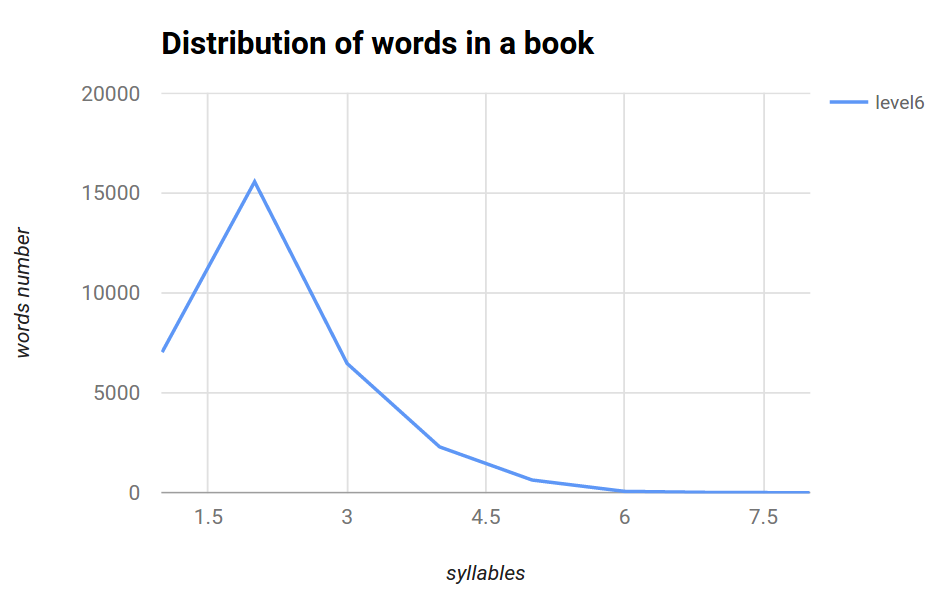
\includegraphics[width=0.6\textwidth]{wordsDistribution} 
\caption{Words in a level 6 book distributing on syllables number}
\end{center}
\end{figure}

Previous researches also shows these criteria has good estimation of the book's readability. For example \cite{flesch}\cite{klare}\cite{chall} used the average sentence length and the average length in syllables to measure the readability of text. 

\section{Data Set}
We have two part of data set: One is from a series book which contains 49 books with readability level labelled by publisher; Another is a huge e-book set from project Gutenberg without readability labelled.
\subsection{Oxford Bookworms Series Book}
The data set we use is the Oxford Bookworms series books\cite{oxford}, which consists of 49 books written in 6 level of readability. These books are re-written by Oxford ELT to fit different readers with reading ability. Below we list the books with their readability level.
\begin{table}[H]
{\renewcommand\arraystretch{1.25}
\begin{tabular}{|l|l|l|} \hline
Readability & \multicolumn{2}{l|}{Books Name} \\ \hline\hline
Level 1 & \multicolumn{2}{p{12cm}|}{\raggedright 
Under The Moon,\,
Love or Money,\,
The Coldest Place on Earth,\,
The Monkey's Paw,\,
The Elephant Man,\,
The Phantom of The Opera,\,
The Witches of Pendle,\,
Mary Queen of Scots} \\ \hline
Level 2 & \multicolumn{2}{p{12cm}|}{
William Shakespeare,\,
Robinson Crusoe,\,
The Love of A King,\,
Five Children and It,\,
Huckleberry Finn,\,
Alice's Adventures in Wonderland,\,
Anne and Green Gables,\,
Dead Man's Island
} \\ \hline
Level 3 & \multicolumn{2}{p{12cm}|}{
A Christmas Carol,\,
The Wind in the Willows,\,
The Star Zoo,\,
Tales of Mystery and Imagination,\,
The Secret Garden,\,
The Call of The Wild,\,
Alice's Adventures in Wonderland,\,
Kidnapped,\,
Tooth and Claw,\,
The Bionte Story,\,
Frankenstein,\,
Chemical Secret,\,
The Prisoner of Zinda,\,
The Piciure of Dorian Gray,\,
} \\ \hline
Level 4 & \multicolumn{2}{p{12cm}|}{
A Tale of Two Cities,\,
The Hound of The Baskervilles,\,
Gulliver' Travels,\,
The Unquiet Grave,\,
Three Men in A Boat,\,
Little Women,\,
Treasure Island,\,
Dr JEKYLL and Mr Hyde,\,
The Thirty-nine Steps,\,
Silas Marner,\,
Black Beauty
} \\ \hline
Level 5 & \multicolumn{2}{p{12cm}|}{
Great Expectations,\,
David Copperfield,\,
Far from the Madding Crowd,\,
Wuthering Heights,\,

} \\ \hline
Level 6 & \multicolumn{2}{p{12cm}|}{
Oliver Twist,\,
Tess,\,
Jane Eyre,\,
Pride and Prejudice

} \\ \hline
\end{tabular}}
\caption{Oxford Bookworms Series Books} \label{tab: testtime}
\end{table}

These levels are all given by Oxford ELT according to the readability of the books. Books in lower level is easier than books in higher level.
\newline
\newline
We get all the books in plain text stored in .txt format file from the Internet. After pre-process, we only retain the alphabets and three symbols space, comma and full stop. These book totally have 649777 words, occupying 5.2MB.

\subsection{Books from Gutenberg}
Gutenberg is a project that offers a great number of free e-books for research use. These books are all real world books taken from free epub books, free kindle books. Since most of the books were previously published by bona fide publishers, and were digitized and proofread by thousands of volunteers, the quality of the books are ensured.
\newline
\newline
In our project, we downloaded 1255 books from Gutenberg website, which is 519.5MB in total. In later section we will test our algorithm on this huge data set to see the speed and space performance of our algorithm.

\subsection{Special Case}
Except for above data set, we also tested our algorithm on an special case, in which the book is extremely difficult. The book we choose is \textit{Wealth of Nation}\cite{wealth}.


%----------------------------------------------------------------------------------------
%	SECTION 3
%----------------------------------------------------------------------------------------
\section{Design}
	To quantify the vague and subjective term readability, we use a score $R$ to represent it. Recall in Section 2.1 we have pointed out 3 important features of texts in book, which are $(a)$ huge vocabulary reduce the readability, $(b)$ difficult words reduce the readability and $(c)$ long sentences reduce the readability. Correspondingly we summarized three reasonable criteria for evaluating the read of a book, as following.
	\begin{enumerate}
		\item \textbf{Number of distinct words}: the distinct words amount in the book $D = |\{w_i\}|$
		\item \textbf{Syllables' variance}: the variance of the syllables of all the words 
			$W = var[syl(w_i)]$ where $syl$ counts the syllables of a word.
		\item \textbf{Average sentence length}: the ratio of the number of words (with repetition) and the number of full stop symbols
			$L = \frac{s}{\textrm{number of full stops}}$.
	\end{enumerate}
	
	We combine these 3 criteria as one $R$ by giving each some proportion and sum them together, but notice that the weight of $D$, $W$ and $L$ does not represents their importance. For example, $D$ is about 100 bigger than $L$ and 1000 bigger than $W$.
	\[R = 0.02D + 5W + L.\]

	To gain the three criteria $D$, $W$ and $L$, we designed three separate parts of our streaming algorithm, which grade on a text stream and
	reflect the corresponding criteria.

	\subsection{Distinct words counting}
		For the first criteria, we only need to count the distinct words in a book. Or equivalently, count the distinct elements
		in a multi-set as a stream. There are lots of algorithms for such problem, e.g. \textit{Hit Counting}, \textit{Adaptive Sampling},
		\textit{Min Count} and \textit{HyperLogLog}.
		The algorithm we used is the well-known HyperLogLog algorithm\cite{hyper}, which is an improved
		minimum-count algorithm.
\newline
\newline
		To be precise, let $n$ be the number of distinct words,
		namely $n = | \{w_1, w_2, \cdots, w_s\} |$ and let these elements be $e_1, e_2, \cdots, e_n$.
		The intuition behind minimum-count algorithms is that each sketch carries information about the desired quantity. For example, when every
		elements $e_j$ is associated with a uniform random variable, e.g. a hash function $h(e_j) \in [0, 1]$, then the expected minimum value
		of $h(e_1), h(e_2), \cdots, h(e_n)$ is $\frac{1}{n + 1}$. The hash function $h$ guarantees that $h(e_j)$ is identical for all the
		appearances of $e_j$. Thus, the existence of duplicates does not affect.
	\newline
	\newline
		And further more, HyperLogLog algorithm is an improvement and offers the better performance. It uses the integer random variables within
		$[0, 2^p]$ (in our design, $p$ equals $32$) instead of real number, which is more computer-friendly. And it counts the largest number
		of the position of the leftmost $1$-bit in binary representation of a number (e.g. $\rho(0001\cdots) = 4$, $\rho(01\cdots) = 2$).
		But actually it is equivalent to count the minimum number, since the more leading zeros a number has, the smaller it is.
		The critical defect of above minimum-count algorithm is that the variance is too large, which causes unstability. One idea is that
		repeat the algorithm via different hash functions and take the mean. And another idea, which we would use in HyperLogLog, is that
		divide all the numbers into $m$ different groups, calculate the answer for each group, and finally take the harmonic mean.
	\newline
	\newline
		By analysis \{{\color{red}ref needed here!!!}\}, we also need to normalize our result with coefficient
		\[ \alpha_m = ( m \int_0^\infty (\log_2(\frac{2 + u}{1 + u}))^m du)^{-1}. \]

		The theoretic relative error of this method is $\pm \frac{1.04}{\sqrt{m}}$. See the implementation section and result section for more detials.

	\subsection{Variance method according to syllables}
		For the second one, basically, we want to do something with the word's syllables. The idea behind is that
		if most words are just one-syllable words, with high probability we could say that it is an easy-reading book.
	\newline
	\newline
		So, firstly we need to calculate the number of syllables of a word. Basic rules for syllabication could help us. However as we known,
		there are many exceptions in the real English world. Such calculation can't be accuracy. Thus we did something much simpler but more
		effective. We simply count the number of vowels as an estimation of the number of syllables.
		Now, for a stream of words, we could give each word a score according to that estimation of the syllables.
	\newline
	\newline
		Naturally, the average of all these socres may give us a good evaluation. But in the practice, just take the mean of these scores is not
		a good measure, as many difficult books have lower evaluation than easy books according to average value.
		The reason is that, even in the difficult book, most
		words are just one-syllable or two-syllable words such as ``a", ``the" and ``of". There isn't a big enough gap between easy one and
		difficult one.
	\newline
	\newline
		However, the variance does. Different from the mean, just a few multiple-syllable words can make nonnegligible contribution to the variance.
	\newline
	\newline
		By the definition, the variance can not be calculated streamingly using limited space. But we can do some tricks as following (let
		$\sigma = \mathbb{E} [x]$).
		\[\begin{array}{lll}
			var(x) & = & \mathbb{E} [(x - \sigma)^2]\\
			& = & \mathbb{E} [x^2 - 2\sigma x + \sigma^2]\\
			& = & \mathbb{E} [x^2] - 2\sigma \mathbb{E} [x] + \mathbb{E} [\sigma^2]\\
			& = & \mathbb{E} [x^2] - 2\sigma^2 + \sigma^2\\
			& = & \mathbb{E} [x^2] - \sigma^2\\
			\end{array}
		\]

		The square of the expected value and the expected value of the square can both be maintained streamingly using only $O(1)$ space and linear
		time.

	\subsection{Average length of sentences}
		The last goal is evaluating the difficulty of structure of each sentence. Obviously, it is not an easy task. Thus, we tried
		some simple ways to solve this problem. The most effective and surprising one is that just take the average length of each sentences.
	\newline
	\newline
		Although, length is very different from difficulty, but it is a good approximate measure. As we know, complicated sentences always
		have subordinate clauses and much more decorated words. Note that length here means the number of words, e.g. $len($``We are students."
		$) = 3$.
	\newline
	\newline
		The algorithm is relatively simple. Just maintain two sketches, one for words, another one for full stop. Thus such algorithm runs
		in linear time and constant space.

%----------------------------------------------------------------------------------------
%	SECTION 4
%----------------------------------------------------------------------------------------
\section{Implementation}
		Some more details of our implementation which is not mentioned in above sections are described here. And the brief pseudocode of
		our implementation are listed below.

        \subsection{Distinct words counting}
            Let $h: \mathcal{W} \rightarrow \{0, 1\}^{32}$ be the hash function hash from words $\mathcal{W}$ to binary $32$-bit integer.
			We implemented our $h$ as following:
				\begin{enumerate}
					\item Choose a random number $b > 26$, and then convert word $v$ into a $b$-based number, e.g. $h(``bob") =
						\overline{bob}_{31} = 
						2 \cdot 31^2 + 15 \cdot 31 + 2$. Note that ``a" should be considered as $1$ instead of $0$. Otherwise there is no
						difference between $h(``a")$ and $h(``aa")$.
					\item Choose three random numbers $k, c, p$, return the value of $k \cdot \overline{v}_b + c \bmod{p}$ as the hash value
						of $h(v)$.
				\end{enumerate}
			It costs linear time on the length of the word.
			\newline
			\newline
            And let $\rho(s)$ be the position of the leftmost $1$-bit of $s$: e.g. $\rho(1\cdots) = 1, \rho(0001\cdots) = 4, \rho(0^K) = K + 1$.
			This function could be simply implemented by enumerating all the binary bits from the highest one to the lowest one, which costs
			$O(\log m)$ time.
			The time complexity and space complexity of this sub-algorithm are $O(s \log m)$ and $O(m)$. Following is the pseudocode.

                \begin{center}
                \begin{algorithmic}
                        \Function{HyperLogLog\_Sketch}{$\mathcal{M}$ : a stream of words from $\mathcal{W}$}
                                \State $M[0], \cdots, M[m - 1]\gets 0$
                                \For {$v \in \mathcal M$}
                                        \State $x \gets h(v)$
                                        \State $j \gets 1 + \langle x_1 x_2 \cdots x_b \rangle_2$
                                        \State $w \gets x_{b + 1}x_{b + 2}\cdots$
                                        \State $M[j] \gets \max(M[j], \rho(w))$
                                \EndFor
                                \State \Return $E \gets \alpha_m m^2 \cdot (\sum\limits^m_{j = 1} 2^{-M[j]})^{-1}$
                        \EndFunction
                \end{algorithmic}
                \end{center}
        \subsection{Variance method according to syllables}
			Let $r : \mathcal{W} \rightarrow \mathbb{N}$ be the function which could calculate the number of syllables of words in $\mathcal{W}$.
			And we need maintain three counters: one for the number of words, one for the linear sum of syllables, and the last one for the
			square sum of syllables.

			But how can we implement such $r$? Roughly, we estimate such number by counting the number of vowels.
			Since according to the basic syllabication rule, each syllable should consist of at least one vowel. But we still implement some
			other exceptional rules, including the tailing voiceless consonant, character ``r" following another vowel,
			and two consecutive vowels. If you are really interested in, please refer to our code implementation.

			The time complexity and space complexity of this sub-algorithm are $O(s)$ and $O(1)$. Following is the pseudocode.

                \begin{center}
                \begin{algorithmic}
                        \Function{Variance\_Sketch}{$\mathcal{M}$ : a stream of words from $\mathcal{W}$}
                                \State $expect, square, n \gets 0$
                                \For {$v \in \mathcal M$}
                                        \State $x \gets r(v)$
                                        \State $square \gets square + x^2$
                                        \State $expect \gets expect + x$
                                        \State $n \gets n + 1$
                                \EndFor
                                \State \Return $E \gets \frac{square}{n} - (\frac{expect}{n})^2$
                        \EndFunction
                \end{algorithmic}
                \end{center}
        \subsection{Average length of sentenses}
			The implementation of this sub-algorithm is quite easy, just maintain the number of words and the number of full stop.
			The time complexity and space complexity of this sub-algorithm are $O(s)$ and $O(1)$. Following is the pseudocode.
                \begin{center}
                \begin{algorithmic}
                        \Function{Length\_Sketch}{$\mathcal{M}$ : a stream of words from $\mathcal{W}$}
                                \State $word, stop \gets 0$
                                \For {$v \in \mathcal M$}
                                        \If {$v$ is a full\ stop}
                                                \State $stop \gets stop + 1$
                                        \Else
                                                \If {$v$ is a word}
                                                        \State $word \gets word + 1$
                                                \EndIf
                                        \EndIf
                                \EndFor
                                \State \Return $E \gets \frac{word}{stop}$
                        \EndFunction
                \end{algorithmic}
                \end{center}


%----------------------------------------------------------------------------------------
%	SECTION 5
%----------------------------------------------------------------------------------------
\section{Results}
We have tested our program on two data sets. While one is labelled with readability level, another does not but contains a big number of books. We tested our accuracy performance by using the Oxford Bookworms data set, while the time and space performance is tested by the Gutenberg data set.
\subsection{Accuracy Performance}
Our algorithm has achieved good estimation of the readability of the books. We applied our algorithm on the Oxford bookworms series books as Figure 2 shows. In the graph, books in y-axis is sorted by their level, so the lower books are more difficult to read. We can see that our $R$ value is growing as the books become more difficult.
\begin{figure}[H]
\begin{center}
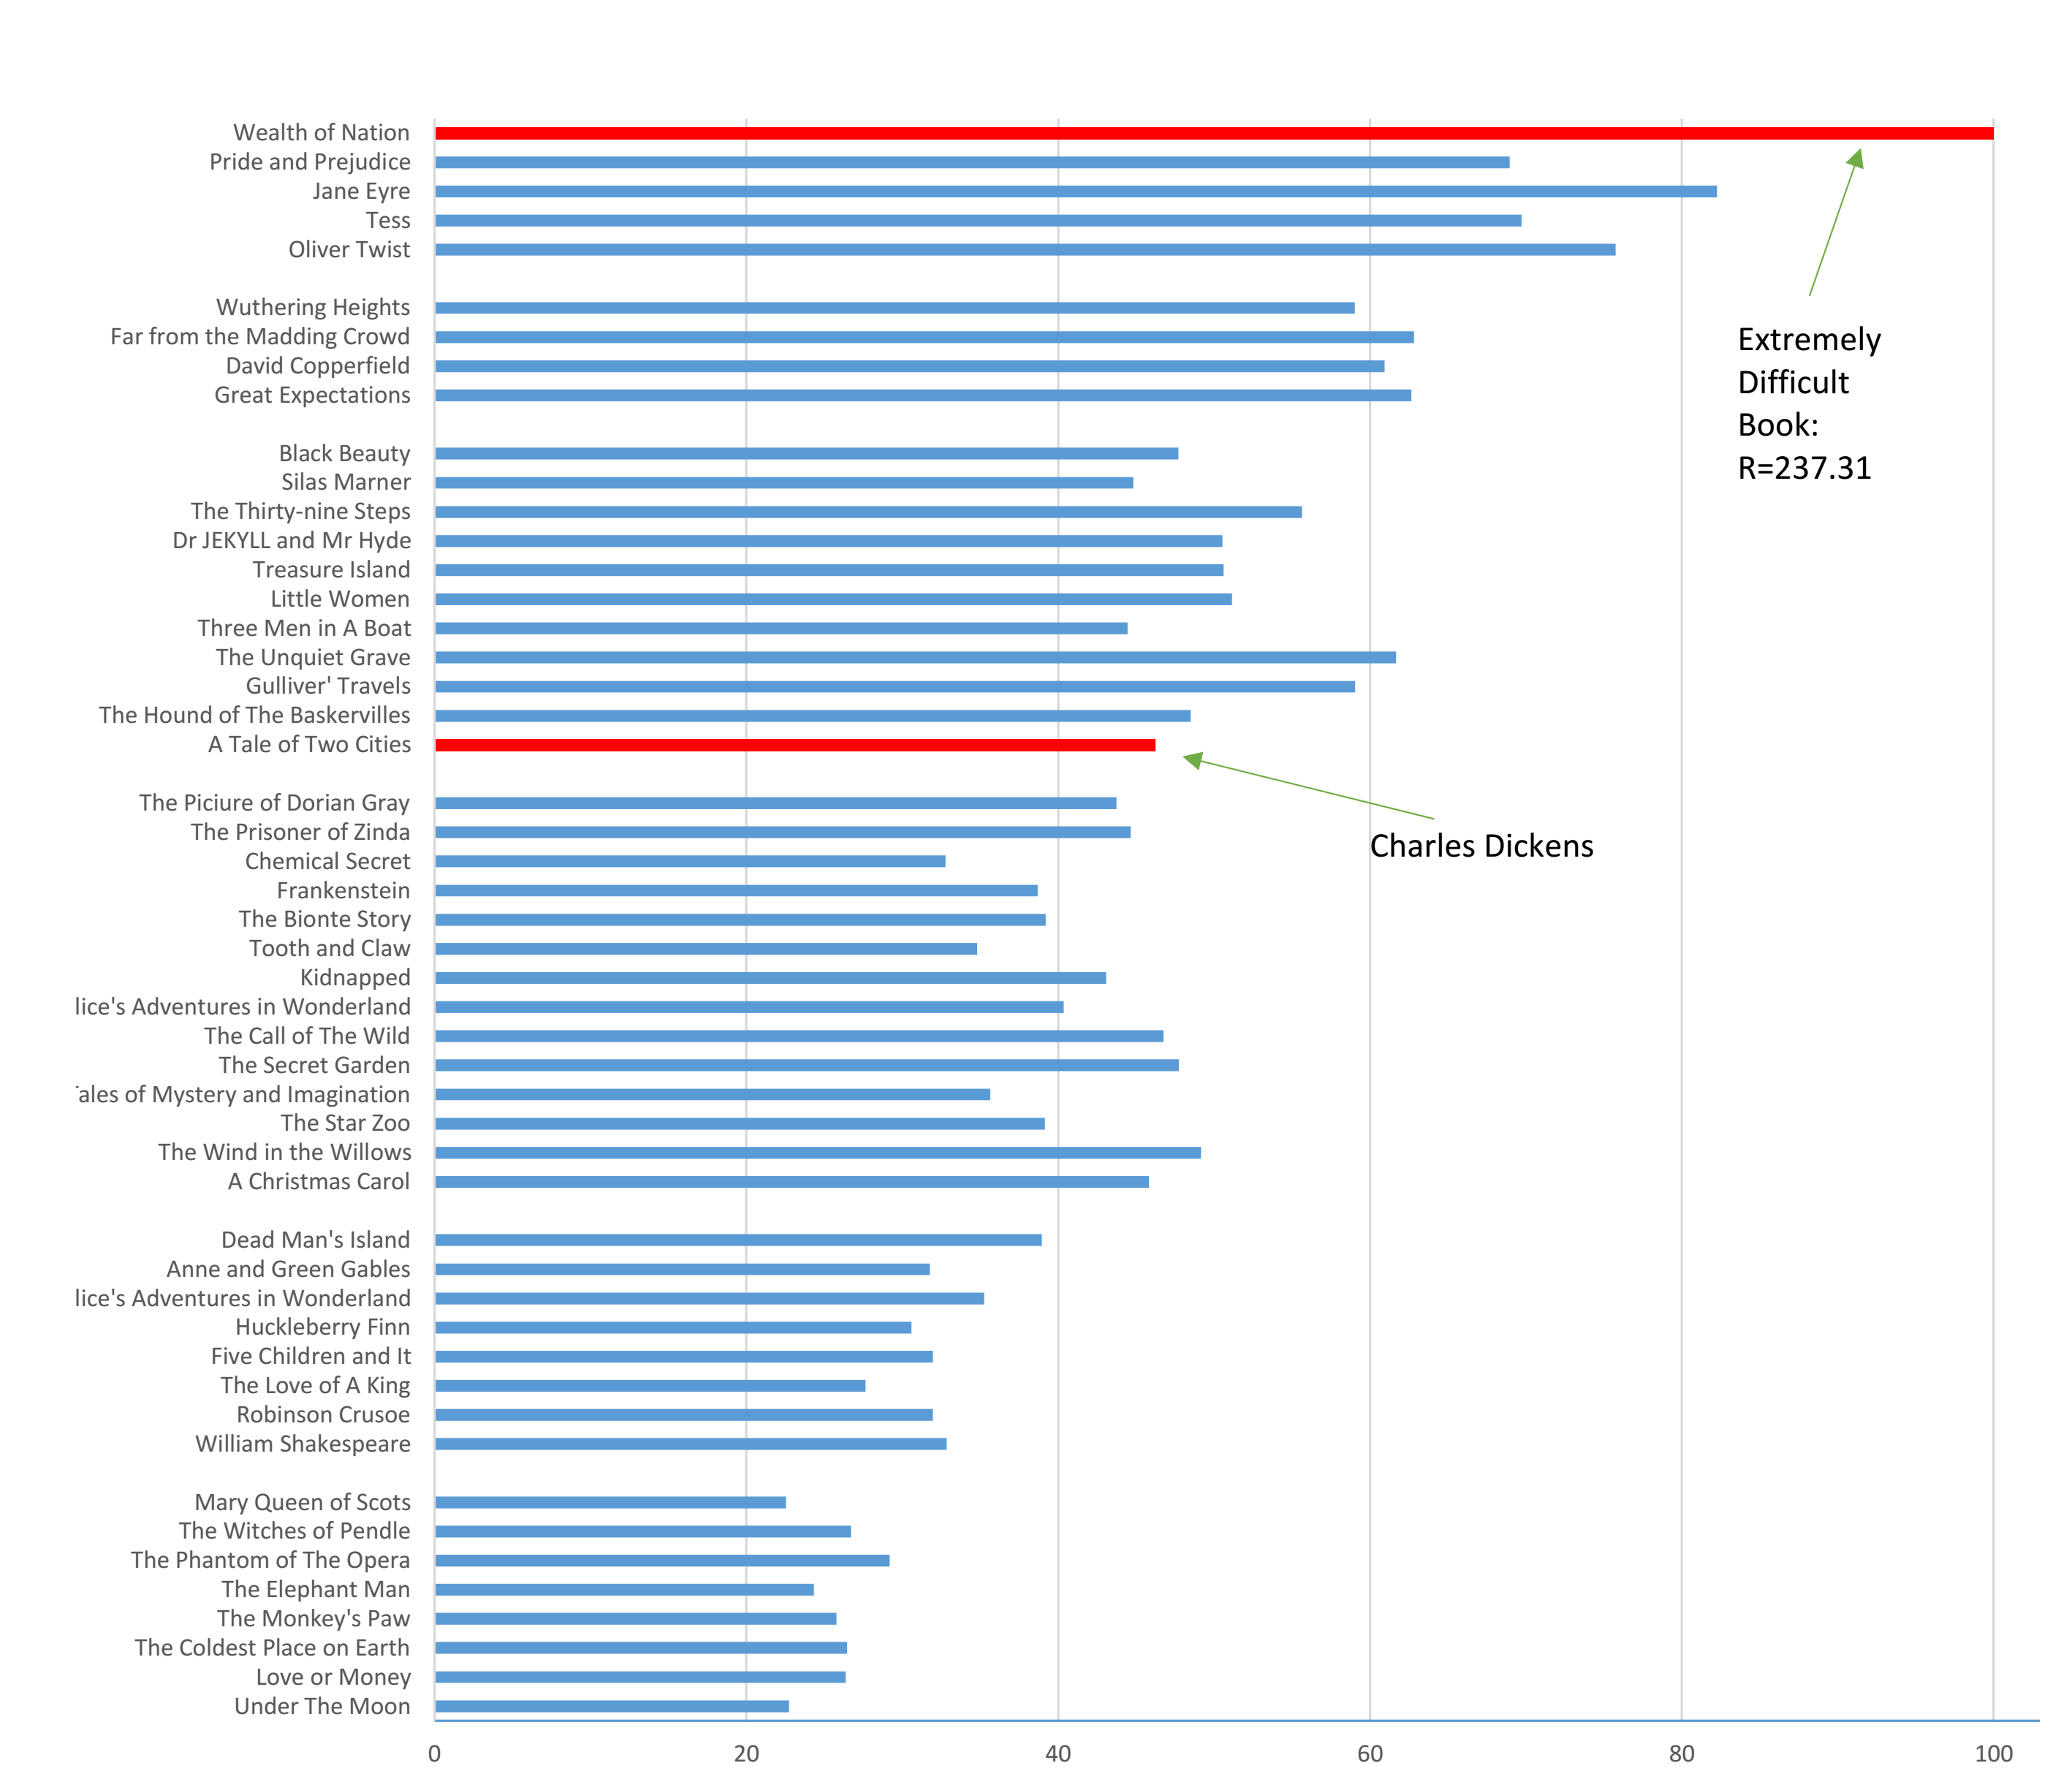
\includegraphics[width=1\textwidth]{50books} 
\caption{50 books R values, y-axis sorted by level (m = 16)}
\end{center}
\end{figure}

Except for Oxford bookworms series book, we have tested other special cases, the book \textit{Wealth of Nation}, which is known to all that this book is very very difficult. We can see is R value in Figure 2, which is much higher than all other books. Another special case is book with long sentence but is not really hard: Charles Dickens's book. We can see his book ranks at the middle of all the books.

\subsection{Space Performance}
We test the space performance by comparing our streaming implementation and non-streaming implementation. We run both of them on the Gutenberg data set. The non-streaming implementation used a C++ STL container \textit{set} to count the distinct value. To test the space of a running program used is not easy. However, not like the time cost, the calculated theoretical space cost is usually consists with the real cost. Here we know the struct of STL container \textit{set} and the data it processed, so we wrote a script to calculate the space overhead of \textit{set}, the value in the non-streaming row is the result.
\begin{table}[H]
\begin{center}
\begin{tabular}{ | m{10em} | m{5em}| m{10em} | m{5em} | m{5em} |} 
\hline
Average s = 6894.3 & m & Space Overhead & Average Accuracy \\ 
\hline
Streaming & 16 & 64 bytes & 95.67\% \\ 
\hline
Streaming & 64 & 256 bytes & 97.63\% \\ 
\hline
Streaming & 256 & 1024 bytes & 98.92\% \\ 
\hline
Streaming & 1024 & 4096 bytes & 99.40\% \\
\hline
Non-Stream & - & 387347 bytes & 100.0\% \\
\hline
\end{tabular}
\end{center}
\caption{Space and Accuracy in Hyper Log Log} \label{tab: testtime}
\end{table}
Table 2 shows the result of streaming and non-streaming methods running on 1155 books. We can see that using the streaming method, only 4096 bytes can reach 99.4\% of the full accuracy. Compare to the non-streaming cost is a big improvement. In our practice, use $m = 16$ is accurate enough.
\subsection{Time Performance}
On the test data set Gutenberg 1155 books, our streaming method reduce the total processing time by 26.07\%. The time is mainly saved by Hyper Log Log algorithm.
\begin{table}[H]
\begin{center}
\begin{tabular}{ | m{10em} | m{10em}| m{10em} | } 
\hline
& Streaming  & Non-Streaming \\ 
\hline
Totall Time & 98.91 second & 130.71 second \\ 
\hline
Input Time & 5.01 second & 4.9 second \\
\hline
Processing Time & 93.00 second & 125.81 second \\
\hline
\end{tabular}
\end{center}
\caption{Time Spend on 1155 books (Data 519.5MB, m = 16)} \label{tab: testtime}
\end{table}
\section{Discussion}
Overall, our project succeed in reflect the readability of a given book by streaming method. Our project shows a great example of applying streaming method to gain more space and time efficiency. And also we should realize this is done by sacrificing certain accuracy. So in reality, not every problem can be solved by streaming. Only those are not sensitive to accuracy and with limited space resources fits the streaming algorithm.
\newline
\newline
Through this project, we also realized convert a solution to streaming method is not easy. There may have no existing streaming method for your problem. Or there may have many different streaming methods for your problem, but you still have to carefully choose them. Or your problem is totally not suitable for streaming. A defect of our project we thought is that although we reduce the space cost greatly, it turns out it may not be so useful. Because modern PC can easily process an arbitrary book with non-streaming method since a book contains only few data. In section 6.2, even the non-streaming method use much more space than streaming method, the overhead still not exceeds 1 MB. And even if you store all the 519MB to memory, it is not a big deal to modern PC. Therefore, thinking for apply a streaming algorithm to a certain system should be careful.
\newline
\newline
We think this is also true for other methods we learned from this class: sub-linear, cache, parallel. We can not streaming or parallel every thing. They are just fit for some certain problem. But once the problem matches the algorithm, the result will be fantastic.


%----------------------------------------------------------------------------------------
%	BIBLIOGRAPHY
%----------------------------------------------------------------------------------------
\newpage


%----------------------------------------------------------------------------------------
\bibliographystyle{plain}

\bibliography{reference}

\end{document}
